\chapter{Dynamická měření}\label{navesti:dynamickaMereni}
Dynamická měření přísunů radonu jsem provedl u tří objektů, viz tab.~\ref{tab:dynMer_prehled}.
\begin{table}[ht]
	\centering
	\caption{Objekty, v nichž jsem provedl dynamická měření. $dt$ značí dobu měření ve dnech (zaokrouhleno na celé dny včetně počátečního a posledního dne). V posledním sloupci je počet zón, na které byl daný objekt rozdělen.}
	\label{tab:dynMer_prehled}
	\begin{tabular}{lllll}
		\toprule
		Objekt & Rozsah měření & $dt$ [dny] & Typ objektu &$N$\\
		\midrule
		Skála 75, okr. Havlíčkův Brod & 23. 5. -- 5. 6. 2019 & 14 & chata & 3\\
		Hálková 980, Humpolec & 5. 6. -- 20. 6. 2019 & 15 & byt & 4\\
		Anglická 574, Dobřichovice & 9. 7. -- 30. 7. 2019 & 22 & rodinný dům & 3\\
		\bottomrule
	\end{tabular}
\end{table}

Vývoj OAR v čase v jednotlivých zónách byl měřen primárně TERA sondami~\cite{tera} a sekundárně měřiči radonu CANARY~\cite{canary}. CANARY měřáky byly použity jako záložní systém, tj. pokud by v některé zóně  TERA sonda selhala, pak by se OAR v této zóně brala z příslušného CANARY měřáku. %Zevrubné informace o těchto detektorech lze dohledat v kapitole~\ref{navesti:radon}.

Dále bylo potřeba měřit vývoj teploty, což je znalost nutná při vyhodnocování množství nasorbovaných indikačních plynů v TD detektorech a k určení hmotnostních koncentrací indikačních plynů  v zónách. K tomuto účelu byly použity dataloggery teploty a vlhkosti testo 174H~\cite{testo}. V případě objektu Hálková 980 byly k určení hmotnostních koncentrací použity teploty naměřené TERA sondami, jelikož v tomto objektu byl osazen pouze jeden datalogger testo 174H (jedná se jednopodlažní byt). 

Pro určení hmotnostních koncentrací indikačních plynů je dále nutno změřit průměrné atmosférické tlaky ve všech zónách. Jejich hodnoty však stačí znát pouze přibližně, protože moc neovlivňují výpočet koncentrací. Proto byly všechny potřebné atmosférické tlaky při vyhodnocování všech objektů brány rovny \SI{100}{kPa}.

Objemy všech objektů byly změřeny laserovým dálkoměrem BOSCH GLM 120 C~\cite{dalkomer}.

Do objektů byly při měřeních umístěny vždy jeden nebo dva zdroje radonu typu RF 2000 (viz podkapitola \ref{navesti:radon_zdroje}). U těchto zdrojů nás pro naše měření zajímají pouze radonové výdejnosti $W$, které představují definované absolutní přísuny radonu do zón, ve kterých jsou zdroje umístěny. Absolutními přísuny radonu je myšleno množství aktivity radonu, jenž se do zón dostane za hodinu, a tedy jejich jednotkou je \si{Bq/hod}. Radonové výdejnosti použitých zdrojů jsou uvedeny v tab.~\ref{tab:dynMer_zdroje}. Podělením $W$ objemem příslušné zóny můžeme dopočítat přísun radonu pocházející od daného zdroje do této zóny. 
\begin{table}[ht]
    \centering
    \caption{ID a radonové výdejnosti $W$ použitých radonových zdrojů typu RF 2000. Jako ID byla použita část výrobního čísla daného zdroje. Přebráno z certifikátů zdrojů, viz příloha~\ref{navesti:priloha_zdroje}.}
    \label{tab:dynMer_zdroje}
    \begin{tabular}{lr}
        \toprule
        ID & $W$ [\si{Bq/hod}]\\
        \midrule
        38 & 15588\\
        37 & 14436\\
        \bottomrule
    \end{tabular}
\end{table}

Před samotnými měřeními přísunů radonu v objektech bylo nejprve nutno provést srovnávací měření TERA sond, jelikož každá sonda má různou odezvu při stejné OAR. O tom pojednává podkapitola~\ref{navesti:dynMer_TERA}. Další podkapitoly obsahují dynamická měření přísunů radonu v uvedených objektech. Je potřeba dávat pozor na to, zdali je značení OAR a přísunů radonu bráno podle podlaží či podle zón. Pokud se jedná objekt, který nelze rozdělit na zóny podle podlaží, pak je značení bráno podle zón, v opačném případě je používáno značení podle podlaží.

\section{TERA sondy}\label{navesti:dynMer_TERA}

Pro dynamická měření přísunů radonu mi byly poskytnuty čtyři TERA sondy s označením 8, 10, 88 a 112. Pro srovnání jejich odezev s reálnou hodnotou OAR byly vloženy do sudu (nádoba válcovitého tvaru) spolu s referenčním monitorem radonu AlphaGuard (ozn. AG)~\cite{alphaguard}. Hodnota OAR z AG byla brána jako reálná hodnota OAR. V obr.~\ref{fig:dynMer_sondySrovnani} jsou zobrazeny naměřené vývoje OAR v čase ze zkoumaných sond a z AG, v tab.~\ref{tab:dynMer_sondy} jsou k vidění nejdůležitější statistiky naměřených dat z každého monitoru.

\begin{figure}[H]
	\centering
	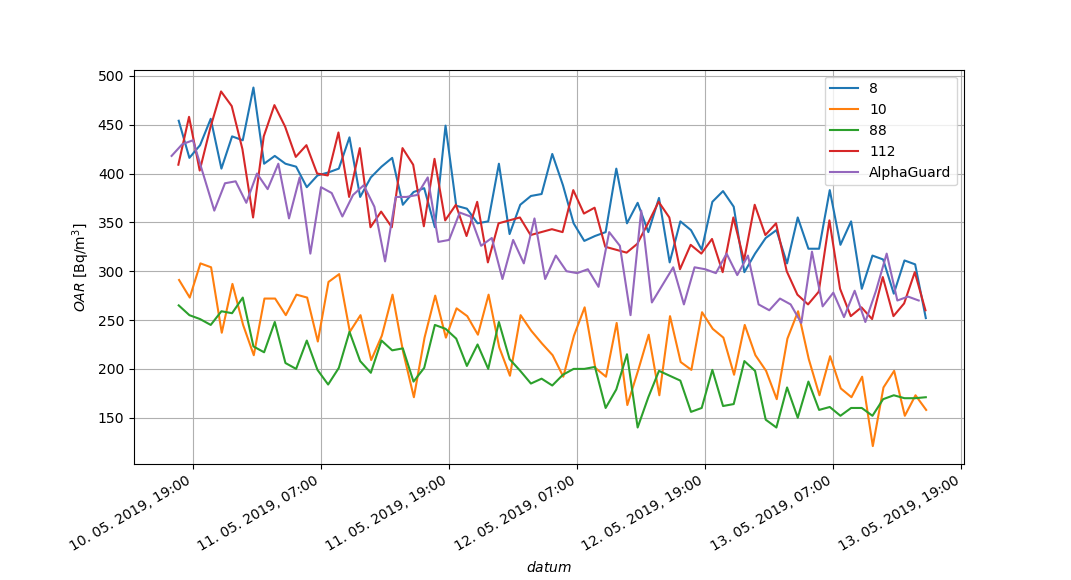
\includegraphics[width=1\linewidth]{images/sondy_srovnani}
	\caption{Vývoj OAR naměřený zkoumanými sondami a AG.}
	\label{fig:dynMer_sondySrovnani}
\end{figure}
\begin{table}[ht]
	\centering
	\caption{Statistiky vývojů OAR naměřených TERA sondami a AG v \si{Bq/m^3}.}
	\label{tab:dynMer_sondy}
	\begin{tabular}{lrrrrrrr}
		\toprule
		ID sondy &  count &  mean    &  min &  25\% &  50\% &  75\% &  max \\
		\midrule
		8          &     71 &   369  &  252 &  337 &  368 &  405 &  488 \\
		10         &     71 &   228  &  121 &  198 &  232 &  256 &  308 \\
		88         &     71 &   198  &  140 &  170 &  198 &  220 &  273 \\
		112        &     71 &   354  &  251 &  318 &  349 &  399 &  484 \\
		\midrule
		AG &     71 &   328  &  247 &  285 &  318 &  373 &  434 \\
		\bottomrule
	\end{tabular}
%&  std
      
%&   47
%&   41
%&   33
%&   58
      
%&   50
\end{table}

Pro opravu odezev byla zavedena pro každou sondu kalibrační konstanta $B$, která je definována následovně:
\begin{equation}
	B=\frac{OAR_A}{OAR_T}\,,
\end{equation}
kde $OAR_A$ je průměrná OAR z hodnot naměřených AG a $OAR_T$ je průměrná OAR z hodnot naměřených příslušnou TERA sondou. Pro získání věrohodné hodnoty koncentrace radonu z naměřené hodnoty danou sondou pak stačí tuto naměřenou hodnotu přenásobit $B$ náležející této sondě.

Relativní nejistoty kalibračních konstant byly odhadnuty na 10~\%. Určené kalibrační konstanty všech sond jsou k nahlédnutí v tab.~\ref{tab:dynMer_sondyB}. %Nejistoty kalibračních konstant určeny nebyly vzhledem k tomu, že se jedná o "veličinu", která se může při různých vnějších podmínkách měnit. Hlavním ovlivňujícím faktorem je velikost aerosolů v měřeném prostředí. Tato nespolehlivost TERA sond v poskytování věrohodných dat je dalším důvodem, proč byly použity měřáky radonu CANARY. Takto můžeme srovnávat data z více zdrojů.
%\begin{figure}[H]
	%\centering
	%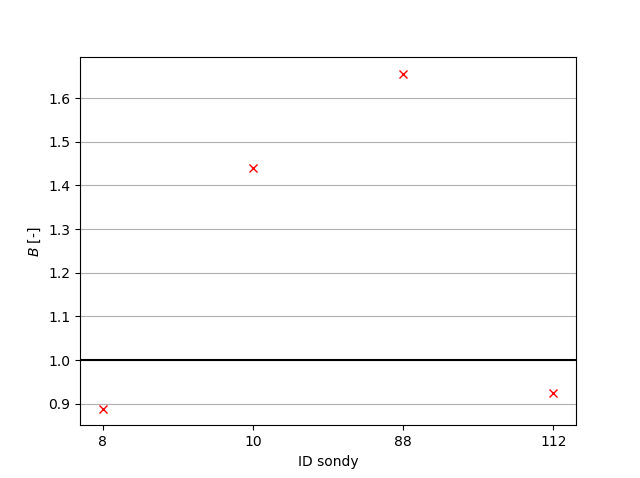
\includegraphics[width=0.7\linewidth]{images/sondy_B}
	%\caption{Kalibrační konstanty proměřených TERA sond. Černou čárou je vyznačen ideální případ, kdy se odezva sondy rovná skutečné OAR (resp. OAR naměřené AlphaGuardem).}
	%\label{fig:dynMer_sondyB}
%\end{figure}
\begin{table}[ht]
	\centering
	\caption{Kalibrační konstanty TERA sond odvozené od referenčního AG. Skutečná hodnota $OAR$ se vypočte ze vztahu $OAR=B\cdot OAR_T$, kde $OAR_T$ je naměřená obj. aktivita radonu danou TERA sondou. Nejistota kalibračních konstant byla odhadnuta na 10~\%.}
	\label{tab:dynMer_sondyB}
	\begin{tabular}{lr}
		\toprule
		ID sondy &     $B$ \\
		\midrule
		8   & 0,889$\pm$0,089\\
		10  & 1,440$\pm$0,140\\
		88  & 1,655$\pm$0,166\\
		112 & 0,925$\pm$0,093\\
		\bottomrule
	\end{tabular}
\end{table}

\section{Objekt Skála 75, okr. Havlíčkův Brod}

Jedná se o chatu se sklepem, přízemím (které zahrnuje verandu) a prvním patrem. Rozdělení na kompartmenty bylo provedeno podle těchto podlaží. Do každého podlaží/zóny byly umístěny vyvíječe dvou typů indikačních plynů. Ve sklepě byly čtyři vyvíječe plynů TMH a TCE, v přízemí šest vyvíječů plynů MDC a MCH a v prvním patře čtyři vyvíječe plynů PCH a PCE. Dále byly umístěny TD detektory: dva do sklepa, šest do přízemí a čtyři do prvního patra. Do sklepa a prvního patra byly umístěny jeden CANARY měřák a jedna TERA sonda, v přízemí byly oba dva typy monitorů dvakrát. Nakonec byly dány do sklepa a přízemí průtočné zdroje radonu typu RF 2000 (do sklepa zdroj s označením 38, do přízemí s označením 37) a byly změřeny objemy. 

To, že jsme umístili do každé ze zón zdroje dvou různých indikačních plynů, umožnilo vyhodnocení měření ventilace vícero způsoby. Při vyhodnocování bylo totiž počítáno pouze s $N=N_p=3$, přičemž byly uvažovány plyny, jejichž zdroje byly v různých zónách (viz pravidla o osazování měřidel, podkapitola~\ref{navesti:prutoky_instalace}). To nám dává osm kombinací trojic použitých plynů a tedy osm různých způsobů vyhodnocení měření ventilaci a následně přísunů radonu.

V příloze~\ref{navesti:priloha_skala75} lze dohledat i vyhodnocené veličiny z měření ventilace a OAR. Je tam také uveden výpočet nejistot průměrných hodnot OAR z dat naměřených TERA sondami (podle informací uvedených v podkapitole~\ref{navesti:radon_TERAnejistota}). 

V následujícím oddíle jsou uvedeny přesně definované přísuny radonu od zdrojů RF 2000 a dále průměrné přísuny radonu vypočítané z naměřených průtoků vzduchu mezi zónami a z OAR naměřených TERA sondami, resp. CANARY měřáky pro všechny kombinace indikačních plynů. V případě TERA sond proběhlo i dynamické vyhodnocení pro určení vývojů $Q_i(t)$, které lze vidět v příloze~\ref{navesti:priloha_skala75_prisuny}, v následujícím oddílu jsou pouze uvedeny zprůměrované hodnoty $Q_i(t)$. V posledním oddílu této kapitoly je zobrazeno zpětné ověření (ve smyslu podkapitoly~\ref{navesti:model_overeni}), navíc jsou tam uvedeny i průměrné OAR naměřené CANARY měřáky a objemové průtoky vzduchu z vyhodnocení měření ventilace objektu při použití kombinace indikačních plynů (TMH, MCH,
PCE).




%\subsection{Použitá měřidla}
%\begin{itemize}
    %\setlength\itemsep{0em}
	%\item 14 vyvíječů (2x TMH, 2x TCE, 3x MDC, 3x MCH, 2x PCE, 2x PCH)
	%\item 12 TD detektorů
	%\item 4 CANARY monitory
	%\item 4 TERA sondy
	%\item 3 TESTO měřiče teploty a vlhkosti
	%\item 2 zdroje radonu
%\end{itemize}

%\subsection{Naměřené OAR, objemy a teploty}

%\begin{table}[H]
    %\centering
    %\caption{Objemy podlaží objektu, průměrné teploty naměřené v každém podlaží dataloggery testo 174H, odhadnuté atmosférické tlaky v každém podlaží a přiřazení číslování kompartmentů jednotlivým podlažím. Význam označení podlaží je vysvětlen v tab. \ref{tab:rovMer_podlazi}.}
    %\label{tab:skala75_objemy}
    %\begin{tabular}{lll}
\toprule
podlazi & $OAR$ [\si{Bq/m^3}] & $V$ [\si{m^3}] \\
\midrule
0 &           1094+/-55 &         40+/-8 \\
1 &            562+/-20 &        84+/-10 \\
2 &              51+/-2 &        97+/-15 \\
\bottomrule
\end{tabular}

%\end{table}
%\begin{figure}[H]
    %\centering
    %\includegraphics[width=1\textwidth]{skala75/OAR_dohromady.png}
    %\caption{Vývoj OAR naměřený TERA sondami po aplikování kalibračních konstant (tab.~\ref{tab:dynMer_sondyB}). Pro další vyhodnocování byly OAR naměřené v přízemí v kuchyni a v ložnici zprůměrovány.}
    %\label{fig:skala75_OAR_dohromady}
%\end{figure}
%\begin{figure}[H]
    %\centering
    %\includegraphics[width=1\textwidth]{skala75/OAR_CANARY.png}
    %\caption{Vývoj OAR naměřený CANARY měřáky.}
    %\label{fig:skala75_OAR_CANARY}
%\end{figure}
%\subsection{Objemové průtoky vzduchu}

%\begin{table}[H]
    %\centering
    %\caption{Přehled použitých indikačních plynů a umístění jejich vyvíječů v objektu. V posledním sloupci jsou celkové odpary plynů ze všech jim odpovídajících vyvíječů.}
    %\label{tab:skala75_indikacniPlyny}
    %\begin{tabular}{lrrrr}
\toprule
ozn. & podlaží& odpar [mg] &    $M$ [g/mol] &    $U$ $\left[\si{\frac{ng}{ppm\cdot min}}\right]$\\
\midrule
TMH & 0 &192,50 &  450,0 &  8,000 \\
TCE & 0 &193,55 &  130,4 &  1,000 \\
MCH & 1 &472,27 &  350,0 &  8,000 \\
MDC & 1 &497,27 &  400,0 &  8,000 \\
PCH & 2 &230,88 &  450,0 &  8,000 \\
PCE & 2 & 96,54 &  165,8 &  1,385 \\
\bottomrule
\end{tabular}

%\end{table}
%\begin{table}[H]
    %\centering
    %\caption{Odezvy TD detektorů $R$ na všechny použité indikační plyny ve všech zónách.}
    %\label{tab:skala75_odezvyTD}
    %\begin{tabular}{lrr}
\toprule
plyn & zóna & $R$ [\si{ng}]               \\
\midrule
MCH & 1 & $  36,0\pm2,3$\\
    & 2 & $395,8\pm16,6$\\
    & 3 & $  50,8\pm2,3$\\
MDC & 1 & $  34,5\pm1,2$\\
    & 2 & $ 304,9\pm7,1$\\
    & 3 & $  47,2\pm1,2$\\
TMH & 1 & $145,3\pm26,0$\\
    & 2 & $  37,5\pm3,9$\\
    & 3 & $  20,2\pm2,4$\\
PCH & 1 & $  20,7\pm2,4$\\
    & 2 & $  26,9\pm0,7$\\
    & 3 & $ 182,2\pm4,6$\\
TCE & 1 & $191,8\pm14,5$\\
    & 2 & $  32,2\pm1,4$\\
    & 3 & $  25,0\pm1,2$\\
PCE & 1 & $     0,0\pm0,0$\\
    & 2 & $   2,6\pm0,1$\\
    & 3 & $ 136,9\pm4,1$\\
\bottomrule
\end{tabular}

%\end{table}

%\begin{table}[H]
    %\centering
    %\caption{Objemové průtoky vzduchu v \si{m^3/hod} pro všechny kombinace aplikovaných indikačních plynů. $n$ je výměna vzduchu vypočtená ze vztahu~\eqref{eq:prutoky_n}, $[n]=\si{1/hod}$.}
    %\label{tab:skala75_prutoky}
%\begin{tabular}{l>{\raggedleft\arraybackslash}p{2.5cm}>{\raggedleft\arraybackslash}p{2.5cm}>{\raggedleft\arraybackslash}p{2.5cm}>{\raggedleft\arraybackslash}p{2.5cm}}
%\toprule
%{} & (TMH, MDC, PCE) & (TMH, MDC, PCH) & (TMH, MCH, PCE) & (TMH, MCH, PCH)\\ 
%\midrule
%$k_{12}$ &12,262$\pm$3,129 &  11,759$\pm$3,078 &  10,188$\pm$2,611 &   9,746$\pm$2,563 \\          
%$k_{13}$ & 0,855$\pm$0,255 &   3,372$\pm$1,013 &   0,908$\pm$0,261 &   3,573$\pm$1,036 \\          
%$k_{21}$ & 4,028$\pm$0,940 &   3,507$\pm$0,847 &   3,220$\pm$0,776 &   2,780$\pm$0,700 \\          
%$k_{23}$ & 1,240$\pm$0,183 &   4,889$\pm$0,724 &   1,025$\pm$0,161 &   4,031$\pm$0,635 \\          
%$k_{31}$ &-0,076$\pm$0,020 &   3,524$\pm$0,958 &  -0,061$\pm$0,016 &   3,611$\pm$0,968 \\          
%$k_{32}$ & 0,931$\pm$0,137 &   5,967$\pm$0,967 &   0,774$\pm$0,117 &   4,945$\pm$0,820 \\          
%&&&&\\
%$k_{1_E}$&21,425$\pm$5,271 &  19,770$\pm$5,057 &  23,244$\pm$5,443 &  21,411$\pm$5,208 \\          
%$k_{2_E}$&44,024$\pm$4,853 &  41,624$\pm$4,833 &  36,712$\pm$4,240 &  34,644$\pm$4,195 \\          
%$k_{3_E}$& 7,712$\pm$0,849 &  24,294$\pm$3,199 &   7,850$\pm$0,853 &  25,127$\pm$3,209 \\          
%$k_{1_I}$&30,590$\pm$6,206 &  27,869$\pm$6,140 &  31,181$\pm$6,093 &  28,339$\pm$6,017 \\          
%$k_{2_I}$&36,099$\pm$5,855 &  32,294$\pm$5,917 &  29,994$\pm$5,043 &  26,764$\pm$5,073 \\          
%$k_{3_I}$& 6,472$\pm$0,916 &  25,525$\pm$3,693 &   6,630$\pm$0,914 &  26,079$\pm$3,658 \\          
%\midrule                                                                              
%$n$      & 0,310$\pm$0,038 &   0,363$\pm$0,042 &   0,287$\pm$0,036 &   0,344$\pm$0,041 \\
%\bottomrule
%\end{tabular}
%\vspace{0.5cm}

%\begin{tabular}{l>{\raggedleft\arraybackslash}p{2.5cm}>{\raggedleft\arraybackslash}p{2.5cm}>{\raggedleft\arraybackslash}p{2.5cm}>{\raggedleft\arraybackslash}p{2.5cm}}
    %\toprule
    %{} & (TCE, MDC, PCE) & (TCE, MDC, PCH) & (TCE, MCH, PCE) & (TCE, MCH, PCH) \\
    %\midrule
%$k_{12}$ & 7,859$\pm$1,288 &   7,286$\pm$1,238 &   6,544$\pm$1,094 &   6,050$\pm$1,047 \\
%$k_{13}$ & 0,893$\pm$0,159 &   3,523$\pm$0,631 &   0,927$\pm$0,162 &   3,647$\pm$0,641 \\
%$k_{21}$ & 1,309$\pm$0,211 &   1,140$\pm$0,195 &   1,049$\pm$0,182 &   0,906$\pm$0,169 \\
%$k_{23}$ & 1,235$\pm$0,180 &   4,874$\pm$0,715 &   1,023$\pm$0,159 &   4,025$\pm$0,628 \\
%$k_{31}$ &-0,025$\pm$0,005 &   1,146$\pm$0,243 &  -0,020$\pm$0,004 &   1,176$\pm$0,245 \\
%$k_{32}$ & 0,922$\pm$0,136 &   6,419$\pm$0,960 &   0,767$\pm$0,116 &   5,330$\pm$0,817 \\
%&&&&\\
%$k_{1_E}$& 2,474$\pm$1,325 &   0,539$\pm$1,320 &   3,713$\pm$1,256 &   1,616$\pm$1,248 \\
%$k_{2_E}$&46,234$\pm$4,862 &  43,556$\pm$4,848 &  38,543$\pm$4,268 &  36,229$\pm$4,226 \\
%$k_{3_E}$& 7,670$\pm$0,848 &  26,236$\pm$3,237 &   7,815$\pm$0,852 &  27,185$\pm$3,242 \\
%$k_{1_I}$& 9,941$\pm$1,867 &   9,061$\pm$1,942 &  10,155$\pm$1,683 &   9,231$\pm$1,776 \\
%$k_{2_I}$&39,997$\pm$5,039 &  35,866$\pm$5,149 &  33,303$\pm$4,414 &  29,780$\pm$4,477 \\
%$k_{3_I}$& 6,439$\pm$0,891 &  25,404$\pm$3,517 &   6,613$\pm$0,889 &  26,019$\pm$3,470 \\
%\midrule                                                                                 
%$n$      & 0,239$\pm$0,028 &   0,298$\pm$0,034 &   0,212$\pm$0,025 &   0,275$\pm$0,031 \\
%\bottomrule
%\end{tabular}
%\end{table}

\subsection{Přísuny radonu}
\begin{table}[H]
    \centering
    \caption{Přesně definované přísuny radonu ze zdrojů v \si{Bq/(m^3\cdot hod)}. Ve druhém sloupci je uvedeno, který zdroj byl umístěn v daném podlaží.}
    \label{tab:skala75_prisunyZdroj}
    \begin{tabular}{ll
        >{\collectcell\num}r<{\endcollectcell}
        @{${}\pm{}$}
        >{\collectcell\num}r<{\endcollectcell}}
        \toprule
        podlaží  &zdroj& \multicolumn{2}{r}{$Q_{zdroj}$}\\
        \midrule
        0 &38&400&51\\
        1 &37&114&13\\
        2 & NE &0&0\\
        \bottomrule
    \end{tabular}
\end{table}

\subsubsection{Vyhodnocení dynamického měření}
\begin{table}[H]
    \centering
    \caption{Průměrné přísuny radonu v \si{Bq/(m^3\cdot hod)} souhrnně pro všechny kombinace indikačních plynů určené zprůměrováním časových vývojů $Q_i(t)$ vypočítaných z dynamického vyhodnocení OAR naměřených TERA sondami. Závislosti $Q_i(t)$ lze vidět v příloze~\ref{navesti:priloha_skala75}.}
    \label{tab:skala75_prisunyDynamicky}
   \begin{tabular}{lrrrr}
\toprule
použité tracery & $Q_0$ $\left[\si{\frac{Bq}{m^3\cdot hod}}\right]$ & $Q_1$ $\left[\si{\frac{Bq}{m^3\cdot hod}}\right]$ & $Q_2$ $\left[\si{\frac{Bq}{m^3\cdot hod}}\right]$ & $Q_3$ $\left[\si{\frac{Bq}{m^3\cdot hod}}\right]$ \\
\midrule
(MDC, PCE, TCE, TMH) & 401+/-383 &    9+/-243 &       97+/-163 &                               -100+/-611 \\
(MDC, MCH, TCE, TMH) & 398+/-356 &   29+/-183 &      101+/-158 &                               -103+/-575 \\
\bottomrule
\end{tabular}

\end{table}
\subsubsection{Vyhodnocení v rovnovážném stavu}
%\begin{table}[H]
    %\centering
    %\caption{Průměrné objemové koncentrace radonu naměřené TERA sondami umístěnými v uvedených podlažích. $\sigma_A$ je nejistota OAR typu A plynoucí ze statistického zpracování naměřených dat, $\sigma_B$ je nejistota OAR typu B plynoucí z ostatních zdrojů (statistika detekce, nejistota měřidla) a $\sigma$ je kombinovaná nejistota OAR. Při určování přísunů radonu v rovnovážném stavu byla použita pouze nejistota typu B, tj. $\sigma_B$. V posledním sloupci je průměrná citlivost TERA sond vypočtená z naměřených dat (tj. z naměřeného počtu impulzů a naměřeného OAR). Tato citlivost byla použita pro výpočet $\sigma_B$.}
    %\label{tab:skala75_OARprumerne}
    %\begin{tabular}{llrrrrr}
%\toprule
%ID sondy&podlaží& OAR [\si{Bq/m^3}]& $\sigma_A$ & $\sigma_B$ &$\sigma$& $\overline{c}$ $\left[\si{\frac{imp}{hod}/\frac{Bq}{m^3}}\right]$\\ 
%\midrule
%8  &0 & 458 & 309 & 33 & 311&0,405\\
%10 &1 & 789 & 485 & 43 & 487&0,433\\
%112&1 & 633 & 282 & 37 & 284&0,464\\
%88 &2 & 276 & 356 & 31 & 358&0,296\\
%\bottomrule
    %\end{tabular}
%\end{table}

%\begin{table}[H]
    %\centering
    %\caption{Průměrné OAR naměřené CANARY měřáky umístěnými v daných podlažích.}
    %\label{tab:skala75_OARprumerne_CANARY}
    %\begin{tabular}{llr}
        %\toprule
        %ID měřáku & podlaží & OAR [\si{Bq/m^3}]\\
        %\midrule
        %1 & 0 & $381\pm38$\\
        %2 & 1 & $419\pm42$\\
        %4 & 1 & $465\pm47$\\
        %3 & 2 & $156\pm16$\\
        %\bottomrule
    %\end{tabular}
%\end{table}

\begin{table}[H]
    \centering
    \caption{Přísuny radonu určené z průměrných hodnot vývojů OAR naměřených TERA sondami. Jednotkou přísunů radonu je \si{Bq/(m^3\cdot hod)}.}
    \label{tab:skala75_prisunyRovnovazne}
   \begin{tabular}{llll}
\toprule
{} & $Q_0$ $\left[\si{\frac{Bq}{m^3\cdot hod}}\right]$ & $Q_1$ $\left[\si{\frac{Bq}{m^3\cdot hod}}\right]$ & $Q_2$ $\left[\si{\frac{Bq}{m^3\cdot hod}}\right]$ \\
\midrule
(TMH, MDC, PCE) &                                          335+/-90 &                                          236+/-42 &                                            18+/-6 \\
(TMH, MDC, PCH) &                                          323+/-88 &                                          231+/-42 &                                           63+/-24 \\
(TMH, MCH, PCE) &                                          347+/-89 &                                          197+/-36 &                                            19+/-6 \\
(TMH, MCH, PCH) &                                          334+/-87 &                                          192+/-35 &                                           70+/-24 \\
(TCE, MDC, PCE) &                                          111+/-28 &                                          249+/-41 &                                            17+/-6 \\
(TCE, MDC, PCH) &                                          108+/-28 &                                          243+/-41 &                                           62+/-23 \\
(TCE, MCH, PCE) &                                          115+/-26 &                                          208+/-35 &                                            19+/-6 \\
(TCE, MCH, PCH) &                                          111+/-27 &                                          203+/-35 &                                           70+/-23 \\
\bottomrule
\end{tabular}

\end{table}

\begin{table}[H]
    \centering
    \caption{Přísuny radonu určené z průměrných hodnot vývojů OAR naměřených CANARY měřáky. Jednotkou přísunů radonu je \si{Bq/(m^3\cdot hod)}.}
    \label{tab:skala75_prisunyRovnovazneCANARY}
   \begin{tabular}{lllll}
\toprule
{} & $Q_1$ $\left[\si{\frac{Bq}{m^3\cdot hod}}\right]$ & $Q_2$ $\left[\si{\frac{Bq}{m^3\cdot hod}}\right]$ & $Q_3$ $\left[\si{\frac{Bq}{m^3\cdot hod}}\right]$ & $Q_4$ $\left[\si{\frac{Bq}{m^3\cdot hod}}\right]$ \\
\midrule
(MDC, PCE, TCE, TMH) &                                         200+/-168 &                                         139+/-356 &                                          75+/-127 &                                         165+/-172 \\
(MDC, MCH, TCE, TMH) &                                          201+/-78 &                                          141+/-75 &                                           76+/-59 &                                          166+/-80 \\
\bottomrule
\end{tabular}

\end{table}

\subsection{Zpětné ověření}

\subsubsection{OAR}
\begin{table}[H]
    \centering
    \caption{Průměrné OAR ve všech podlažích vypočítané pomocí rovnice~\eqref{eq:maticovy_zapis_rovnovaha} za použití průtoků vzduchu z tab.~\ref{tab:skala75_prutoky} a přísunů radonu pocházejících od zdrojů RF 2000 (tab.~\ref{tab:skala75_prisunyZdroj}) a průměrné OAR naměřené CANARY měřáky.}
    \label{tab:skala75_OAR_zpetne}
    \begin{tabular}{lrrr}
        \toprule
  použité tracery  & $a_1$ [\si{Bq/m^3}] &  $a_2$ [\si{Bq/m^3}]& $a_3$ [\si{Bq/m^3}] \\
        \midrule
(TMH, MDC, PCE) & $ 496\pm121$ & $410\pm72$ & $103\pm25$ \\
(TMH, MDC, PCH) & $ 496\pm119$ & $410\pm72$ & $107\pm26$ \\
(TMH, MCH, PCE) & $ 495\pm120$ & $467\pm83$ & $102\pm25$ \\
(TMH, MCH, PCH) & $ 495\pm118$ & $467\pm82$ & $107\pm26$ \\
(TCE, MDC, PCE) & $1417\pm333$ & $518\pm85$ & $209\pm50$ \\
(TCE, MDC, PCH) & $1416\pm338$ & $518\pm86$ & $219\pm50$ \\
(TCE, MCH, PCE) & $1415\pm319$ & $574\pm96$ & $209\pm49$ \\
(TCE, MCH, PCH) & $1415\pm324$ & $574\pm96$ & $218\pm49$ \\
\midrule
       naměřené & $381\pm\ \,38$ & $442\pm32$ & $156\pm16$ \\
        \bottomrule
    \end{tabular}
\end{table}

\subsubsection{Objemové průtoky vzduchu}

\begin{table}[H]
    \centering
    \caption{V prvních řádcích těchto tabulek označených \emph{zpětně} jsou průtoky vzduchu z dané zóny do ostatních zón a infiltrace této zóny vypočítané z rovnice~\eqref{eq:maticovy_zapis_rovnovaha} za využití znalosti ostatních průtoků vzduchu pro kombinaci indikačních plynů (TMH, MCH, PCE), viz tab.~\ref{tab:skala75_prutoky}, přísunů radonu pocházejících od zdrojů RF 2000 (tab.~\ref{tab:skala75_prisunyZdroj}) a průměrných OAR naměřených CANARY měřáky. V druhých řádcích tabulek označených \emph{měření} jsou pro srovnání uvedené příslušné průtoky vzduchu z tab.~\ref{tab:skala75_prutoky}. V (a) je zájmovou zónou první zóna, v (b) druhá zóna a v (c) třetí zóna.}
    \label{tab:skala75_prutoky_zpetne}
    \begin{subtable}{\textwidth}
        \centering
        \caption{}
        \begin{tabular}{l>{\collectcell\num}r<{\endcollectcell}@{${}\pm{}$}>{\collectcell\num}r<{\endcollectcell}>{\collectcell\num}r<{\endcollectcell}@{${}\pm{}$}>{\collectcell\num}r<{\endcollectcell}>{\collectcell\num}r<{\endcollectcell}@{${}\pm{}$}>{\collectcell\num}r<{\endcollectcell}>{\collectcell\num}r<{\endcollectcell}@{${}\pm{}$}>{\collectcell\num}r<{\endcollectcell}}
\toprule
{} & \multicolumn{2}{r}{$k_{12}$ [\si{m^3/hod}]} & \multicolumn{2}{r}{$k_{13}$ [\si{m^3/hod}]} & \multicolumn{2}{r}{$k_{1_E}$ [\si{m^3/hod}]} & \multicolumn{2}{r}{$k_{1_I}$ [\si{m^3/hod}]} \\
\midrule
zpětně &                                 1,09&0,16 &                                 1,00&0,18 &                                 8,36&0,67 &                                 7,83&0,91 \\
měření &                                 2,32&0,38 &                                 0,29&0,09 &                                22,05&2,53 &                                21,52&2,60 \\
\bottomrule
\end{tabular}

    \end{subtable}
    \vspace{1em}

    \begin{subtable}{\textwidth}
        \centering
        \caption{}
        \begin{tabular}{lrrrrr}
\toprule
{} & $k_{21}$ [\si{m^3/hod}] & $k_{23}$ [\si{m^3/hod}] & $k_{24}$ [\si{m^3/hod}] & $k_{2_E}$ [\si{m^3/hod}] & $k_{2_I}$ [\si{m^3/hod}] \\
\midrule
zpětně &$97\pm107 $&      $10\pm20 $&                $-22\pm98 $&                 $26\pm31 $&                 $33\pm41 $\\
měření &$ 43\pm\ \,15 $&    $1\pm\ \,2 $&                $ 22\pm13 $&                 $ 11\pm\ \,4 $&                 $18\pm28 $  \\
\bottomrule
\end{tabular}

    \end{subtable}
    \vspace{1em}

    \begin{subtable}{\textwidth}
        \centering
        \caption{}
        \begin{tabular}{lrrrr}
\toprule
{} & $k_{31}$ [\si{m^3/hod}] & $k_{32}$ [\si{m^3/hod}] & $k_{3E}$ [\si{m^3/hod}] & $k_{3I}$ [\si{m^3/hod}] \\
\midrule
zpětně &          -24.45+/-17.34 &            1.34+/-16.37 &           27.71+/-20.50 &           26.49+/-20.50 \\
měření &            -0.06+/-0.02 &             0.77+/-0.12 &             7.85+/-0.85 &             6.63+/-0.91 \\
\bottomrule
\end{tabular}

    \end{subtable}
\end{table}

\subsection{Diskuze}
V diskuzi nejprve srovnáme průměrné přísuny radonu z dynamického a rovnovážného vyhodnocení (tabulky~\ref{tab:skala75_prisunyDynamicky} a \ref{tab:skala75_prisunyRovnovazne}), poté přísuny určené z OAR naměřených TERA sondami a CANARY měřáky (tabulky~\ref{tab:skala75_prisunyRovnovazne} a \ref{tab:skala75_prisunyRovnovazneCANARY}) a následně tyto vypočítané přísuny se známými přísuny od zdrojů (tab.~\ref{tab:skala75_prisunyZdroj}). Při argumentaci také využijeme tabulky~\ref{tab:skala75_OAR_zpetne} a \ref{tab:skala75_prutoky_zpetne} se zpětným ověřením OAR a objemových průtoků vzduchu z $Q_{zdroj}$.

\subsubsection{Srovnání dynamického a rovnovážného vyhodnocení}
Z uvedených tabulek je zřejmé, že zprůměrováním vývojů $Q_i(t)$ dostaneme v podstatě stejné hodnoty jako při rovnovážném vyhodnocení, což bylo očekáváno. Neshodování hodnot by ukazovalo na nějakou chybu v kódu.

\subsubsection{Srovnání použití OAR z TERA sond a z CANARY měřáků}



\subsection{Závěr}

\section{Objekt Hálková 980, Humpolec}
Jedná se o byt s ložnicí, obývacím pokojem, kuchyní s WC, špajzem a předsíní. Za zóny byly brány obývací pokoj, ložnice, koupelna s WC a kuchyň. Špajz a předsín nebyly zahrnuty do žádné ze zón.

Bylo použito dvacet vyvíječů pěti různých indikačních plynů, čtyři vyvíječe pro daný plyn. Do obývacího pokoje byly umístěny vyvíječe s MDC plynem, do ložnice vyvíječe s MCH a PCE plyny, do koupelny s TCE plynem a do kuchyně s TMH plynem.

TD detektory byly po dvojicích umístěny do každé ze zón kromě koupelny, kam byl umístěn pouze jeden TD detektor. Poslední TD detektor byl umístěn do špajzu, protože původně bylo zamýšleno brát jako jednu zónu koupelnu a špajz. %PORUŠENÍ PRAVIDEL OSAZOVÁNÍ MĚŘIDEL!!!!

Do každé zóny byly umístěny jedna TERA sonda a jeden CANARY měřák. Do obývacího pokoje byl umístěn radonový zdroj s označením 38 (dle tab.~\ref{tab:dynMer_zdroje}). 

V dalších oddílech jsou uvedena použitá měřidla, naměřené hodnoty OAR, objemů a teplot. Následují vypočítané veličiny, které bylo potřeba určit pro výpočet přísunů radonu a určené přísuny radonu a zpětné ověření pomocí $Q_{zdroj}$.  
%\subsection{Použitá měřidla}

%\begin{itemize}
    %\setlength\itemsep{0em}
	%\item 20 vyvíječů (4x MDC, 4x MCH, 4x PCE, 4x TCE, 4x TMH)
	%\item 8 TD detektorů
	%\item 4 CANARY monitory
	%\item 4 TERA sondy
	%\item 3 TESTO měřiče teploty a vlhkosti
	%\item 1 zdroj radonu
%\end{itemize}

%\subsection{Naměřené OAR, objemy a teploty}

%\begin{table}[H]
    %\centering
    %\caption{Přiřazení číslování kompartmentů jednotlivým podlažím, objemy všech zón objektu, průměrné teploty naměřené v každém zóně TERA sondami, odhadnuté atmosférické tlaky v každém zóně a průměrné OAR naměřené TERA sondami ($OAR_T$) a CANARY měřáky ($OAR_C$). OAR jsou uvedené v \si{Bq/m^3}.}
    %\label{tab:halkova980_objemy}
    %\begin{tabular}{lll}
\toprule
podlazi & $OAR$ [\si{Bq/m^3}] & $V$ [\si{m^3}] \\
\midrule
0 &           1094+/-55 &         40+/-8 \\
1 &            562+/-20 &        84+/-10 \\
2 &              51+/-2 &        97+/-15 \\
\bottomrule
\end{tabular}

%\end{table}
%\begin{figure}[H]
    %\centering
    %\includegraphics[width=1\textwidth]{halkova980/OAR_dohromady.png}
    %\caption{Vývoj OAR naměřený TERA sondami po aplikování kalibračních konstant (tab.~\ref{tab:dynMer_sondyB}).}
    %\label{fig:halkova980_OAR_dohromady}
%\end{figure}
%\begin{figure}[H]
    %\centering
    %\includegraphics[width=1\textwidth]{halkova980/OAR_CANARY.png}
    %\caption{Vývoj OAR naměřený CANARY měřáky.}
    %\label{fig:halkova980_OAR_CANARY}
%\end{figure}

%\subsection{Objemové průtoky vzduchu}

%\begin{table}[H]
    %\centering
    %\caption{Přehled použitých indikačních plynů a umístění jejich vyvíječů v objektu. V posledním sloupci jsou celkové odpary plynů ze všech jim odpovídajících vyvíječů.}
    %\label{tab:halkova980_indikacniPlyny}
    %\begin{tabular}{lrrrr}
\toprule
ozn. & podlaží& odpar [mg] &    $M$ [g/mol] &    $U$ $\left[\si{\frac{ng}{ppm\cdot min}}\right]$\\
\midrule
TMH & 0 &192,50 &  450,0 &  8,000 \\
TCE & 0 &193,55 &  130,4 &  1,000 \\
MCH & 1 &472,27 &  350,0 &  8,000 \\
MDC & 1 &497,27 &  400,0 &  8,000 \\
PCH & 2 &230,88 &  450,0 &  8,000 \\
PCE & 2 & 96,54 &  165,8 &  1,385 \\
\bottomrule
\end{tabular}

%\end{table}
%\begin{table}[H]
    %\centering
    %\caption{Odezvy TD detektorů $R$ na všechny použité indikační plyny ve všech zónách.}
    %\label{tab:halkova980_odezvyTD}
    %\begin{tabular}{lrr}
\toprule
plyn & zóna & $R$ [\si{ng}]               \\
\midrule
MCH & 1 & $  36,0\pm2,3$\\
    & 2 & $395,8\pm16,6$\\
    & 3 & $  50,8\pm2,3$\\
MDC & 1 & $  34,5\pm1,2$\\
    & 2 & $ 304,9\pm7,1$\\
    & 3 & $  47,2\pm1,2$\\
TMH & 1 & $145,3\pm26,0$\\
    & 2 & $  37,5\pm3,9$\\
    & 3 & $  20,2\pm2,4$\\
PCH & 1 & $  20,7\pm2,4$\\
    & 2 & $  26,9\pm0,7$\\
    & 3 & $ 182,2\pm4,6$\\
TCE & 1 & $191,8\pm14,5$\\
    & 2 & $  32,2\pm1,4$\\
    & 3 & $  25,0\pm1,2$\\
PCE & 1 & $     0,0\pm0,0$\\
    & 2 & $   2,6\pm0,1$\\
    & 3 & $ 136,9\pm4,1$\\
\bottomrule
\end{tabular}

%\end{table}

%\begin{table}[H]
    %\centering
    %\caption{Objemové průtoky vzduchu mezi zónami v \si{m^3/hod} a výměna vzduchu $n$ v \si{hod^{-1}}.}
    %\label{tab:halkova980_prutoky}
    %\begin{tabular}{l
        >{\collectcell\num}r<{\endcollectcell}
        @{${}\pm{}$}
        >{\collectcell\num}r<{\endcollectcell}
        >{\collectcell\num}r<{\endcollectcell}
        @{${}\pm{}$}
        >{\collectcell\num}r<{\endcollectcell}
}
%\begin{tabular}{l>{\raggedleft\arraybackslash}p{2.5cm}>{\raggedleft\arraybackslash}p{2.5cm}}
\toprule
%{} & (MDC, PCE, TCE, TMH) & (MDC, MCH, TCE, TMH) \\
{} & \multicolumn{2}{r}{(MDC, PCE,} & \multicolumn{2}{r}{(MDC, MCH,} \\
{} & \multicolumn{2}{r}{TCE, TMH)} &   \multicolumn{2}{r}{TCE, TMH)} \\
\midrule
$k_{12}$          &    12,2&4,9 &          40,4&13,4   \\
$k_{13}$          &     4,8&8,9 &           11,9&8,2   \\
$k_{14}$          &   96,0&35,9 &          92,9&34,0   \\
$k_{21}$          &   31,3&27,5 &          40,5&14,8   \\
$k_{23}$          &    17,9&7,9 &            4,4&3,3   \\
$k_{24}$          &   13,8&24,1 &          19,7&12,7   \\
$k_{31}$          &   63,4&26,0 &          62,6&26,1   \\
$k_{32}$          &     1,9&2,8 &            6,2&8,9   \\
$k_{34}$          &   46,9&24,3 &          46,5&23,9   \\
$k_{41}$          &   76,3&37,1 &          74,6&37,7   \\
$k_{42}$          &     4,1&4,1 &          13,6&13,2   \\
$k_{43}$          &    18,0&9,7 &           20,4&9,9   \\
&\multicolumn{2}{r}{}&\multicolumn{2}{r}{}\\
$k_{1_E}$          &   72,6&18,6 &          45,3&11,8   \\
$k_{2_E}$          &  -39,9&15,3 &           12,1&4,6   \\
$k_{3_E}$          &  -27,3&12,3 &          -31,5&8,8   \\
$k_{4_E}$          &   50,9&18,7 &          41,7&13,4   \\
$k_{1_I}$          &   14,7&67,4 &          12,7&62,2   \\
$k_{2_I}$          &    5,0&41,0 &          16,6&29,1   \\
$k_{3_I}$          &   44,2&40,8 &          47,1&39,8   \\
$k_{4_I}$          &   -7,5&65,6 &          -8,8&61,4   \\
\midrule
$n$  &     0,4&0,2 &            0,4&0,1   \\   
\bottomrule
\end{tabular}

    
    
    
    
    
    
    
    
    
    
    
    
    
    
    
    
    
    
    
    
    


%\end{table}

\subsection{Přísuny radonu}

\begin{table}[H]
    \centering
    \caption{Přesně definované přísuny radonu ze zdrojů v \si{Bq/(m^3\cdot hod)}. Ve druhém sloupci je uvedeno, který zdroj byl umístěn v dané zóně.}
    \label{tab:halkova980_prisunyZdroj}
    \begin{tabular}{ll
        >{\collectcell\num}r<{\endcollectcell}
        @{${}\pm{}$}
        >{\collectcell\num}r<{\endcollectcell}
    }
        \toprule
        zóna &zdroj  & \multicolumn{2}{r}{$Q_{zdroj}$}\\
        \midrule
        1 &38& 332&64\\
        2 &NE    & 0&0   \\
        3 &NE    & 0&0   \\
        4 &NE    & 0&0   \\
        \bottomrule
    \end{tabular}
\end{table}
%\begin{table}[H]
    %\centering
    %\caption{Statistiky vypočítaných přísunů radonu $Q$ do jednotlivých podlaží.}
    %\label{tab:halkova980_prisuny}
    %\begin{tabular}{lrrr}
\toprule
{} &  $Q_0$ $\left[\si{\frac{Bq}{m^3\cdot hod}}\right]$ &  $Q_1$ $\left[\si{\frac{Bq}{m^3\cdot hod}}\right]$ &  $Q_2$ $\left[\si{\frac{Bq}{m^3\cdot hod}}\right]$ \\
\midrule
count &                                                284 &                                                284 &                                                284 \\
mean  &  3035 &      4367 &     677 \\
std   &  2122 &      2579 &    1470 \\
min   &                                                652 &                                                319 &                                               -934 \\
25%   &                                               1377 &                                               2000 &                                               -224 \\
50%   &                                               2397 &                                               4104 &                                                 11 \\
75%   &                                               3830 &                                               6310 &                                               1389 \\
max   &                                               9130 &                                               9673 &                                               4902 \\
\bottomrule
\end{tabular}

%\end{table}
\begin{table}[H]
    \centering
    \caption{Průměrné přísuny radonu do zón (ne podlaží!) pro všechny možné kombinace indikačních plynů za použití průměrných hodnot vývojů OAR naměřených TERA sondami (rovnovážné vyhodnocení).}
    \label{tab:halkova980_prisunyRovnovazne}
    \begin{tabular}{llll}
\toprule
{} & $Q_0$ $\left[\si{\frac{Bq}{m^3\cdot hod}}\right]$ & $Q_1$ $\left[\si{\frac{Bq}{m^3\cdot hod}}\right]$ & $Q_2$ $\left[\si{\frac{Bq}{m^3\cdot hod}}\right]$ \\
\midrule
(TMH, MDC, PCE) &                                          335+/-90 &                                          236+/-42 &                                            18+/-6 \\
(TMH, MDC, PCH) &                                          323+/-88 &                                          231+/-42 &                                           63+/-24 \\
(TMH, MCH, PCE) &                                          347+/-89 &                                          197+/-36 &                                            19+/-6 \\
(TMH, MCH, PCH) &                                          334+/-87 &                                          192+/-35 &                                           70+/-24 \\
(TCE, MDC, PCE) &                                          111+/-28 &                                          249+/-41 &                                            17+/-6 \\
(TCE, MDC, PCH) &                                          108+/-28 &                                          243+/-41 &                                           62+/-23 \\
(TCE, MCH, PCE) &                                          115+/-26 &                                          208+/-35 &                                            19+/-6 \\
(TCE, MCH, PCH) &                                          111+/-27 &                                          203+/-35 &                                           70+/-23 \\
\bottomrule
\end{tabular}

\end{table}

\begin{table}[H]
    \centering
    \caption{Průměrné přísuny radonu do zón pro všechny možné kombinace indikačních plynů vypočtené z průměrných hodnot vývojů OAR naměřených CANARY měřáky.}
    \label{tab:halkova980_prisunyRovnovazneCANARY}
    \begin{tabular}{lllll}
\toprule
{} & $Q_1$ $\left[\si{\frac{Bq}{m^3\cdot hod}}\right]$ & $Q_2$ $\left[\si{\frac{Bq}{m^3\cdot hod}}\right]$ & $Q_3$ $\left[\si{\frac{Bq}{m^3\cdot hod}}\right]$ & $Q_4$ $\left[\si{\frac{Bq}{m^3\cdot hod}}\right]$ \\
\midrule
(MDC, PCE, TCE, TMH) &                                         200+/-168 &                                         139+/-356 &                                          75+/-127 &                                         165+/-172 \\
(MDC, MCH, TCE, TMH) &                                          201+/-78 &                                          141+/-75 &                                           76+/-59 &                                          166+/-80 \\
\bottomrule
\end{tabular}

\end{table}

\subsection{Zpětné ověření}

\subsubsection{OAR}
\begin{table}[H]
    \centering
    \caption{Průměrné OAR ve všech zónách vypočítané pomocí rovnice~\eqref{eq:maticovy_zapis_rovnovaha} za použití průtoků vzduchu z tab.~\ref{tab:halkova980_prutoky} a přísunů radonu pocházejících od zdrojů RF 2000 (tab.~\ref{tab:halkova980_prisunyZdroj}) a průměrné OAR naměřené CANARY měřáky.}
    \label{tab:halkova980_OAR_zpetne}
    \begin{tabular}{lllll}
\toprule
{} & $Q_1$ $\left[\si{\frac{Bq}{m^3\cdot hod}}\right]$ & $Q_2$ $\left[\si{\frac{Bq}{m^3\cdot hod}}\right]$ & $Q_3$ $\left[\si{\frac{Bq}{m^3\cdot hod}}\right]$ & $Q_4$ $\left[\si{\frac{Bq}{m^3\cdot hod}}\right]$ \\
\midrule
(MDC, PCE, TCE, TMH) &                                         200+/-168 &                                         139+/-356 &                                          75+/-127 &                                         165+/-172 \\
(MDC, MCH, TCE, TMH) &                                          201+/-78 &                                          141+/-75 &                                           76+/-59 &                                          166+/-80 \\
\bottomrule
\end{tabular}

\end{table}

\subsubsection{Objemové průtoky vzduchu}
\begin{table}[H]
    \centering
    \caption{V prvních řádcích těchto tabulek označených \emph{zpětně} jsou průtoky vzduchu z dané zóny do ostatních zón a infiltrace této zóny vypočítané z rovnice~\eqref{eq:maticovy_zapis_rovnovaha} za využití znalosti ostatních průtoků vzduchu pro kombinaci indikačních plynů (MDC, MCH, TCE, TMH), viz tab.~\ref{tab:halkova980_prutoky}, přísunů radonu pocházejících od zdrojů RF 2000 (tab.~\ref{tab:halkova980_prisunyZdroj}) a průměrných OAR naměřených CANARY měřáky. V druhých řádcích tabulek označených \emph{měření} jsou pro srovnání uvedené příslušné průtoky vzduchu z tab.~\ref{tab:halkova980_prutoky}. V (a) je zájmovou zónou první zóna, v (b) druhá zóna, v (c) třetí zóna a v (d) čtvrtá zóna.}
    \label{tab:halkova980_prutoky_zpetne}
    \begin{subtable}{\textwidth}
        \centering
        \caption{}
        \begin{tabular}{l>{\collectcell\num}r<{\endcollectcell}@{${}\pm{}$}>{\collectcell\num}r<{\endcollectcell}>{\collectcell\num}r<{\endcollectcell}@{${}\pm{}$}>{\collectcell\num}r<{\endcollectcell}>{\collectcell\num}r<{\endcollectcell}@{${}\pm{}$}>{\collectcell\num}r<{\endcollectcell}>{\collectcell\num}r<{\endcollectcell}@{${}\pm{}$}>{\collectcell\num}r<{\endcollectcell}}
\toprule
{} & \multicolumn{2}{r}{$k_{12}$ [\si{m^3/hod}]} & \multicolumn{2}{r}{$k_{13}$ [\si{m^3/hod}]} & \multicolumn{2}{r}{$k_{1_E}$ [\si{m^3/hod}]} & \multicolumn{2}{r}{$k_{1_I}$ [\si{m^3/hod}]} \\
\midrule
zpětně &                                 1,09&0,16 &                                 1,00&0,18 &                                 8,36&0,67 &                                 7,83&0,91 \\
měření &                                 2,32&0,38 &                                 0,29&0,09 &                                22,05&2,53 &                                21,52&2,60 \\
\bottomrule
\end{tabular}

    \end{subtable}
    \vspace{1em}

    \begin{subtable}{\textwidth}
        \centering
        \caption{}
        \begin{tabular}{lrrrrr}
\toprule
{} & $k_{21}$ [\si{m^3/hod}] & $k_{23}$ [\si{m^3/hod}] & $k_{24}$ [\si{m^3/hod}] & $k_{2_E}$ [\si{m^3/hod}] & $k_{2_I}$ [\si{m^3/hod}] \\
\midrule
zpětně &$97\pm107 $&      $10\pm20 $&                $-22\pm98 $&                 $26\pm31 $&                 $33\pm41 $\\
měření &$ 43\pm\ \,15 $&    $1\pm\ \,2 $&                $ 22\pm13 $&                 $ 11\pm\ \,4 $&                 $18\pm28 $  \\
\bottomrule
\end{tabular}

    \end{subtable}
    \vspace{1em}

    \begin{subtable}{\textwidth}
        \centering
        \caption{}
        \begin{tabular}{lrrrr}
\toprule
{} & $k_{31}$ [\si{m^3/hod}] & $k_{32}$ [\si{m^3/hod}] & $k_{3E}$ [\si{m^3/hod}] & $k_{3I}$ [\si{m^3/hod}] \\
\midrule
zpětně &          -24.45+/-17.34 &            1.34+/-16.37 &           27.71+/-20.50 &           26.49+/-20.50 \\
měření &            -0.06+/-0.02 &             0.77+/-0.12 &             7.85+/-0.85 &             6.63+/-0.91 \\
\bottomrule
\end{tabular}

    \end{subtable}

    \begin{subtable}{\textwidth}
        \centering
        \caption{}
        \begin{tabular}{lrrrrr}
\toprule
{} & $k_{41}$ [\si{m^3/hod}] & $k_{42}$ [\si{m^3/hod}] & $k_{43}$ [\si{m^3/hod}] & $k_{4E}$ [\si{m^3/hod}] & $k_{4I}$ [\si{m^3/hod}] \\
\midrule
zpětně &                120+/-66 &                -10+/-26 &                 16+/-13 &                 48+/-19 &                 11+/-58 \\
měření &                 83+/-37 &                 14+/-13 &                   9+/-5 &                 38+/-12 &                  0+/-56 \\
\bottomrule
\end{tabular}

    \end{subtable}
\end{table}

\subsection{Diskuze}

\subsection{Závěr}

\section{Objekt Anglická 574, Dobřichovice}
Jedná se o rodinný dům se sklepem, přízemím a prvním patrem. Při měření byla brána jednotlivá podlaží jako zóny. 

%\subsection{Použitá měřidla}
%\begin{itemize}
    %\setlength\itemsep{0em}
	%\item 12 vyvíječů (4x MCH, 4x MDC, 4x PCH)
	%\item 12 TD detektorů
	%\item 2 blank TD detektory 
	%\item 4 CANARY monitory
	%\item 4 TERA sondy
	%\item 3 TESTO měřiče teploty a vlhkosti
	%\item 2 zdroje radonu
%\end{itemize}

%\subsection{Naměřené OAR, objemy a teploty}

%\begin{table}[H]
    %\centering
    %\caption{Objemy všech podlaží objektu, průměrné teploty naměřené v každém podlaží TERA sondami, odhadnuté atmosférické tlaky v každém podlaží, průměrné OAR naměřené TERA sondami ($OAR_T$) a CANARY měřáky ($OAR_C$) a přiřazení číslování kompartmentů jednotlivým podlažím. OAR jsou uvedené v \si{Bq/m^3}.}
    %\label{tab:anglicka574_objemy}
    %\begin{tabular}{lll}
\toprule
podlazi & $OAR$ [\si{Bq/m^3}] & $V$ [\si{m^3}] \\
\midrule
0 &           1094+/-55 &         40+/-8 \\
1 &            562+/-20 &        84+/-10 \\
2 &              51+/-2 &        97+/-15 \\
\bottomrule
\end{tabular}

%\end{table}
%\begin{figure}[H]
    %\centering
    %\includegraphics[width=1\textwidth]{anglicka574/OAR_dohromady.png}
    %\caption{Vývoj OAR naměřený TERA sondami po aplikování kalibračních konstant (tab.~\ref{tab:dynMer_sondyB}).}
    %\label{fig:anglicka574_OAR_dohromady}
%\end{figure}
%\begin{figure}[H]
    %\centering
    %\includegraphics[width=1\textwidth]{anglicka574/OAR_CANARY.png}
    %\caption{Vývoj OAR naměřený CANARY měřáky.}
    %\label{fig:anglicka574_OAR_CANARY}
%\end{figure}

%\subsection{Objemové průtoky vzduchu}

%\begin{table}[H]
    %\centering
    %\caption{Přehled použitých indikačních plynů a umístění jejich vyvíječů v objektu. V posledním sloupci jsou celkové odpary plynů ze všech jim odpovídajících vyvíječů.}
    %\label{tab:anglicka574_indikacniPlyny}
    %\begin{tabular}{lrrrr}
\toprule
ozn. & podlaží& odpar [mg] &    $M$ [g/mol] &    $U$ $\left[\si{\frac{ng}{ppm\cdot min}}\right]$\\
\midrule
TMH & 0 &192,50 &  450,0 &  8,000 \\
TCE & 0 &193,55 &  130,4 &  1,000 \\
MCH & 1 &472,27 &  350,0 &  8,000 \\
MDC & 1 &497,27 &  400,0 &  8,000 \\
PCH & 2 &230,88 &  450,0 &  8,000 \\
PCE & 2 & 96,54 &  165,8 &  1,385 \\
\bottomrule
\end{tabular}

%\end{table}
%\begin{table}[H]
    %\centering
    %\caption{Odezvy TD detektorů $R$ na všechny použité indikační plyny ve všech zónách.}
    %\label{tab:anglicka574_odezvyTD}
    %\begin{tabular}{lrr}
\toprule
plyn & zóna & $R$ [\si{ng}]               \\
\midrule
MCH & 1 & $  36,0\pm2,3$\\
    & 2 & $395,8\pm16,6$\\
    & 3 & $  50,8\pm2,3$\\
MDC & 1 & $  34,5\pm1,2$\\
    & 2 & $ 304,9\pm7,1$\\
    & 3 & $  47,2\pm1,2$\\
TMH & 1 & $145,3\pm26,0$\\
    & 2 & $  37,5\pm3,9$\\
    & 3 & $  20,2\pm2,4$\\
PCH & 1 & $  20,7\pm2,4$\\
    & 2 & $  26,9\pm0,7$\\
    & 3 & $ 182,2\pm4,6$\\
TCE & 1 & $191,8\pm14,5$\\
    & 2 & $  32,2\pm1,4$\\
    & 3 & $  25,0\pm1,2$\\
PCE & 1 & $     0,0\pm0,0$\\
    & 2 & $   2,6\pm0,1$\\
    & 3 & $ 136,9\pm4,1$\\
\bottomrule
\end{tabular}

%\end{table}

%\begin{table}[H]
    %\centering
    %\caption{Objemové průtoky vzduchu mezi zónami v \si{m^3/hod} a výměna vzduchu $n$ v \si{hod^{-1}}.}
    %\label{tab:anglicka574_prutoky}
    %\begin{tabular}{lllll}
\toprule
{} &            0 &          1 &              2 & vnější prostředí \\
\midrule
0                &            0 &  1.3+/-0.4 &  0.033+/-0.029 &           45+/-8 \\
1                &    2.5+/-0.7 &          0 &    0.47+/-0.16 &           23+/-4 \\
2                &  0.14+/-0.12 &  1.3+/-0.4 &              0 &       16.2+/-2.9 \\
vnější prostředí &       44+/-8 &     23+/-4 &     17.1+/-2.9 &                0 \\
\bottomrule
\end{tabular}

%\end{table}

\subsection{Přísuny radonu}

\begin{table}[H]
    \centering
    \caption{Přesně definované přísuny radonu ze zdrojů v \si{Bq/(m^3\cdot hod)}. Ve druhém sloupci je uvedeno, ve kterém podlaží byly zdroje umístěny.}
    \label{tab:anglicka574_prisunyZdroj}
    \begin{tabular}{ll
        >{\collectcell\num}r<{\endcollectcell}
        @{${}\pm{}$}
        >{\collectcell\num}r<{\endcollectcell}}
        \toprule
        podlaží  &zdroj& \multicolumn{2}{r}{$Q_{zdroj}$}\\
        \midrule
        0 &38 \& 37&455&90\\
        1 & NE &0&0\\
        2 & NE &0&0\\
        \bottomrule
    \end{tabular}
\end{table}

%\begin{figure}[ht]
    %\begin{subfigure}{\textwidth}
        %\centering
        %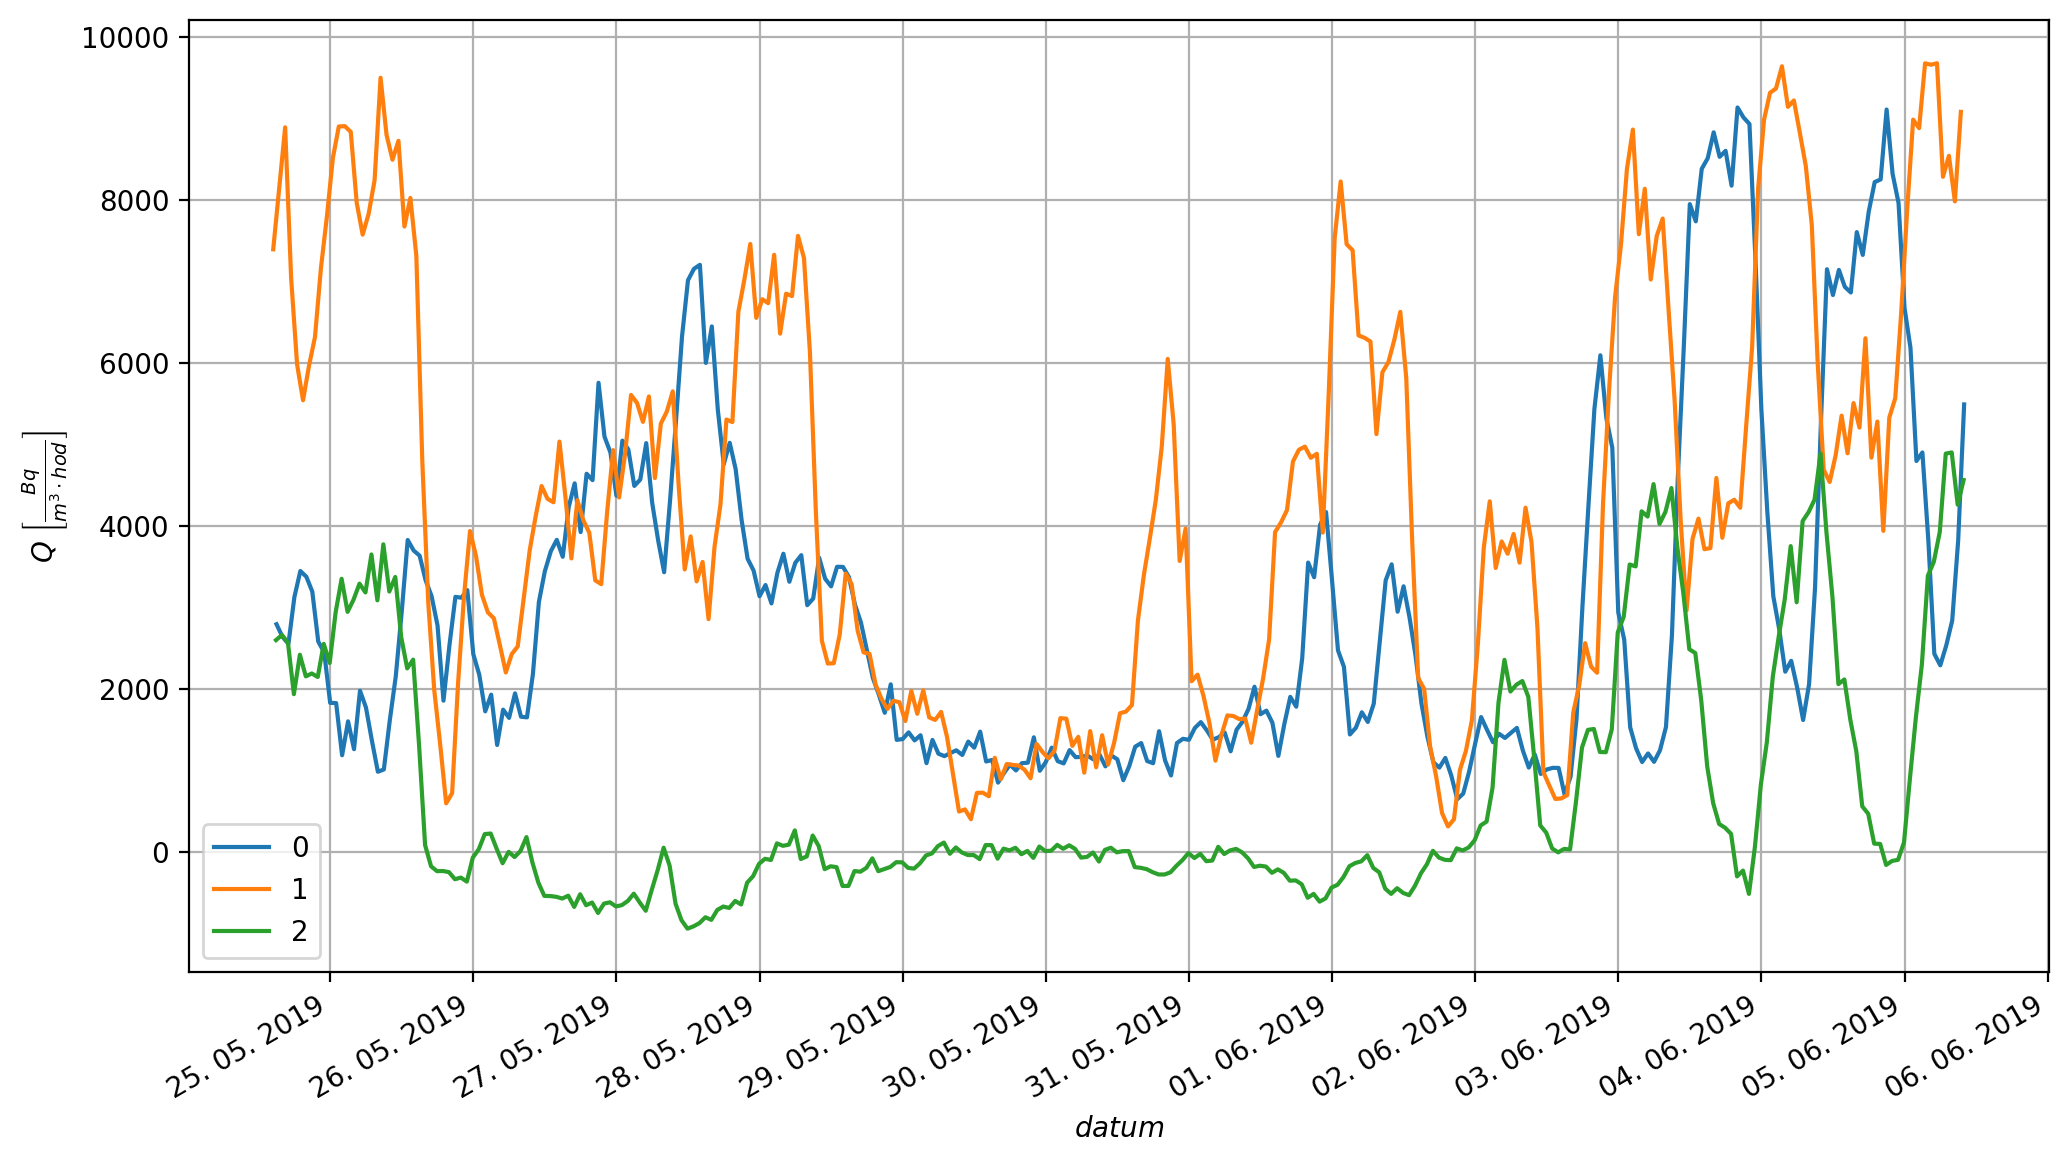
\includegraphics[width=\textwidth]{anglicka574/prisuny.png}
        %\caption{}
        %\label{fig:anglicka574_prisuny}
    %\end{subfigure}
    %\begin{subfigure}{\textwidth}
        %\centering
        %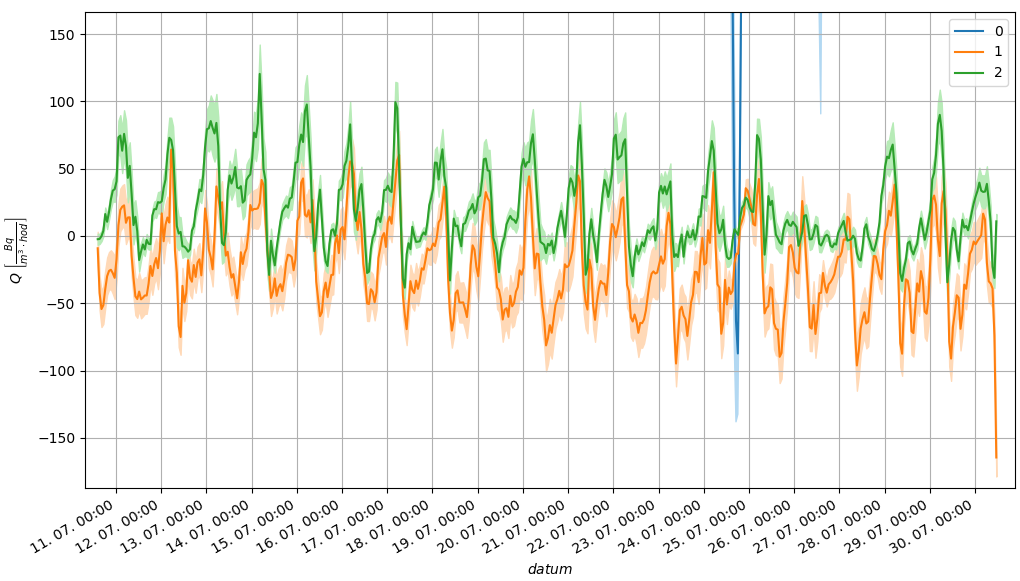
\includegraphics[width=\textwidth]{anglicka574/prisuny_zoom.png}
        %\caption{}
        %\label{fig:anglicka574_prisunyZoom}
    %\end{subfigure}
    %\caption{V (a) jsou určené časové vývoje přísunů radonu do jednotlivých podlaží. V (b) jsou přiblížené přísuny radonu do přízemí a prvního patra. Oblasti označené zesvětlenou barvou značí nejistotu přísunů radonu při faktoru pokrytí $k=1$.}
%\end{figure}
%\begin{table}[H]
    %\centering
    %\caption{Statistiky vypočítaných přísunů radonu $Q$ do jednotlivých podlaží.}
    %\label{tab:anglicka574_prisuny}
    %\begin{tabular}{lrrr}
\toprule
{} &  $Q_0$ $\left[\si{\frac{Bq}{m^3\cdot hod}}\right]$ &  $Q_1$ $\left[\si{\frac{Bq}{m^3\cdot hod}}\right]$ &  $Q_2$ $\left[\si{\frac{Bq}{m^3\cdot hod}}\right]$ \\
\midrule
count &                                                284 &                                                284 &                                                284 \\
mean  &  3035 &      4367 &     677 \\
std   &  2122 &      2579 &    1470 \\
min   &                                                652 &                                                319 &                                               -934 \\
25%   &                                               1377 &                                               2000 &                                               -224 \\
50%   &                                               2397 &                                               4104 &                                                 11 \\
75%   &                                               3830 &                                               6310 &                                               1389 \\
max   &                                               9130 &                                               9673 &                                               4902 \\
\bottomrule
\end{tabular}

%\end{table}
\begin{table}[H]
    \centering
    \caption{Průměrné přísuny radonu do všech podlaží z rovnovážného vyhodnocení za použití dat z TERA sond.}
    \label{tab:anglicka574_prisunyRovnovazne}
    \begin{tabular}{rrr}
        \toprule
        $Q_0$ $\left[\si{\frac{Bq}{m^3\cdot hod}}\right]$& $Q_1$ $\left[\si{\frac{Bq}{m^3\cdot hod}}\right]$ & $Q_2$ $\left[\si{\frac{Bq}{m^3\cdot hod}}\right]$\\
        \midrule
        $1042\pm233$ & $-22\pm12$ & $19\pm9$\\
        \bottomrule
    \end{tabular}
\end{table}
\begin{table}[H]
    \centering
    \caption{Průměrné přísuny radonu do všech podlaží z rovnovážného vyhodnocení za použití dat z CANARY měřáků.}
    \label{tab:anglicka574_prisunyRovnovazneCANARY}
    \begin{tabular}{rrr}
        \toprule
        $Q_0$ $\left[\si{\frac{Bq}{m^3\cdot hod}}\right]$& $Q_1$ $\left[\si{\frac{Bq}{m^3\cdot hod}}\right]$ & $Q_2$ $\left[\si{\frac{Bq}{m^3\cdot hod}}\right]$\\
        \midrule
        $1057\pm245$ & $-31\pm13$ & $21\pm7$\\
        \bottomrule
    \end{tabular}
\end{table}

\subsection{Zpětné ověření}
\subsubsection{OAR}
\begin{table}[H]
    \centering
    \caption{Průměrné OAR ve všech podlažích vypočítané pomocí rovnice~\eqref{eq:maticovy_zapis_rovnovaha} za použití průtoků vzduchu z tab.~\ref{tab:anglicka574_prutoky} a přísunů radonu pocházejících od zdrojů RF 2000 (tab.~\ref{tab:anglicka574_prisunyZdroj}) a průměrné OAR naměřené CANARY měřáky.}
    \label{tab:anglicka574_OAR_zpetne}
    \begin{tabular}{lrrr}
        \toprule
        & $a_0$ [\si{Bq/m^3}] &  $a_1$ [\si{Bq/m^3}]& $a_2$ [\si{Bq/m^3}]\\
        \midrule
       vypočítané & $1200\pm360$    & $84\pm29$ & $22\pm\ \,8$\\
       naměřené & $2770\pm196$ & $92\pm\ \,9$& $98\pm10$\\
        \bottomrule
    \end{tabular}
\end{table}
\subsubsection{Objemové průtoky vzduchu}

\begin{table}[H]
    \centering
    \caption{V prvních řádcích těchto tabulek označených \emph{zpětně} jsou průtoky vzduchu z dané zóny do ostatních zón a infiltrace této zóny vypočítané z rovnice~\eqref{eq:maticovy_zapis_rovnovaha} za využití znalosti ostatních průtoků vzduchu (viz tab.~\ref{tab:anglicka574_prutoky}), přísunů radonu pocházejících od zdrojů RF 2000 (tab.~\ref{tab:anglicka574_prisunyZdroj}) a průměrných OAR naměřených CANARY měřáky. V druhých řádcích tabulek označených \emph{měření} jsou pro srovnání uvedené příslušné průtoky vzduchu z tab.~\ref{tab:anglicka574_prutoky}. V (a) je zájmovou zónou první zóna, v (b) druhá zóna a v (c) třetí zóna.}
    \label{tab:anglicka574_prutoky_zpetne}
    \begin{subtable}{\textwidth}
        \centering
        \caption{}
        \begin{tabular}{l>{\collectcell\num}r<{\endcollectcell}@{${}\pm{}$}>{\collectcell\num}r<{\endcollectcell}>{\collectcell\num}r<{\endcollectcell}@{${}\pm{}$}>{\collectcell\num}r<{\endcollectcell}>{\collectcell\num}r<{\endcollectcell}@{${}\pm{}$}>{\collectcell\num}r<{\endcollectcell}>{\collectcell\num}r<{\endcollectcell}@{${}\pm{}$}>{\collectcell\num}r<{\endcollectcell}}
\toprule
{} & \multicolumn{2}{r}{$k_{12}$ [\si{m^3/hod}]} & \multicolumn{2}{r}{$k_{13}$ [\si{m^3/hod}]} & \multicolumn{2}{r}{$k_{1_E}$ [\si{m^3/hod}]} & \multicolumn{2}{r}{$k_{1_I}$ [\si{m^3/hod}]} \\
\midrule
zpětně &                                 1,09&0,16 &                                 1,00&0,18 &                                 8,36&0,67 &                                 7,83&0,91 \\
měření &                                 2,32&0,38 &                                 0,29&0,09 &                                22,05&2,53 &                                21,52&2,60 \\
\bottomrule
\end{tabular}

    \end{subtable}
    \vspace{1em}

    \begin{subtable}{\textwidth}
        \centering
        \caption{}
        \begin{tabular}{lrrrrr}
\toprule
{} & $k_{21}$ [\si{m^3/hod}] & $k_{23}$ [\si{m^3/hod}] & $k_{24}$ [\si{m^3/hod}] & $k_{2_E}$ [\si{m^3/hod}] & $k_{2_I}$ [\si{m^3/hod}] \\
\midrule
zpětně &$97\pm107 $&      $10\pm20 $&                $-22\pm98 $&                 $26\pm31 $&                 $33\pm41 $\\
měření &$ 43\pm\ \,15 $&    $1\pm\ \,2 $&                $ 22\pm13 $&                 $ 11\pm\ \,4 $&                 $18\pm28 $  \\
\bottomrule
\end{tabular}

    \end{subtable}
    \vspace{1em}

    \begin{subtable}{\textwidth}
        \centering
        \caption{}
        \begin{tabular}{lrrrr}
\toprule
{} & $k_{31}$ [\si{m^3/hod}] & $k_{32}$ [\si{m^3/hod}] & $k_{3E}$ [\si{m^3/hod}] & $k_{3I}$ [\si{m^3/hod}] \\
\midrule
zpětně &          -24.45+/-17.34 &            1.34+/-16.37 &           27.71+/-20.50 &           26.49+/-20.50 \\
měření &            -0.06+/-0.02 &             0.77+/-0.12 &             7.85+/-0.85 &             6.63+/-0.91 \\
\bottomrule
\end{tabular}

    \end{subtable}
\end{table}

\subsection{Diskuze}

\subsection{Závěr}

\section{Shrnutí}
toto bude obsahovat přehledové tabulky obsahující určené přísuny radonu a dulezite poznatky z diskuzi a zaveru
\begin{table}
    \centering
    \caption{(TMH, MCH, PCE), (MDC, MCH, TCE, TMH)}
    \label{tab:dynMer_shrnuti}
    \begin{tabular}{l
        >{\collectcell\num}r<{\endcollectcell}
        @{${}\pm{}$}
        >{\collectcell\num}r<{\endcollectcell}
        >{\collectcell\num}r<{\endcollectcell}
        @{${}\pm{}$}
        >{\collectcell\num}r<{\endcollectcell}
        >{\collectcell\num}r<{\endcollectcell}
        @{${}\pm{}$}
        >{\collectcell\num}r<{\endcollectcell}
        >{\collectcell\num}r<{\endcollectcell}
        @{${}\pm{}$}
        >{\collectcell\num}r<{\endcollectcell}
    }
        \toprule
        {}& \multicolumn{2}{r}{$Q_1$} & \multicolumn{2}{r}{$Q_2$} & \multicolumn{2}{r}{$Q_3$} & \multicolumn{2}{r}{$Q_4$} \\
        \midrule

Skála 75 &   301&78 & 115&24 &   9&3 &  \multicolumn{2}{r}{}\\
Hálková 980 & 445&241 & -86&104 & 38&84 & -152&351 \\
Anglická 574 & 1057&245 & -31&13 & 21&7 &\multicolumn{2}{r}{}\\
\bottomrule
    \end{tabular}
\end{table}
